\documentclass[onecolumn,10pt]{jhwhw}

\usepackage{epsfig} %% for loading postscript figures
\usepackage{amsmath}
\usepackage{graphicx}
\usepackage{grffile}
\usepackage{pdfpages}
\usepackage{algpseudocode}
\usepackage{wrapfig}
\usepackage{booktabs}
\usepackage{multicol}

% Default fixed font does not support bold face
\DeclareFixedFont{\ttb}{T1}{txtt}{bx}{n}{12} % for bold
\DeclareFixedFont{\ttm}{T1}{txtt}{m}{n}{12}  % for normal

% Custom colors
\usepackage{color}
\usepackage{listings}
\usepackage{framed}
\usepackage{caption}
\usepackage{bm}
\captionsetup[lstlisting]{font={small,tt}}

\definecolor{mygreen}{rgb}{0,0.6,0}
\definecolor{mygray}{rgb}{0.5,0.5,0.5}
\definecolor{mymauve}{rgb}{0.58,0,0.82}

\lstset{ %
  backgroundcolor=\color{white},   % choose the background color; you must add \usepackage{color} or \usepackage{xcolor}
  basicstyle=\ttfamily\footnotesize, % the size of the fonts that are used for the code
  breakatwhitespace=false,         % sets if automatic breaks should only happen at whitespace
  % breaklines=true,                 % sets automatic line breaking
  captionpos=b,                    % sets the caption-position to bottom
  commentstyle=\color{mygreen},    % comment style
  deletekeywords={...},            % if you want to delete keywords from the given language
  escapeinside={\%*}{*)},          % if you want to add LaTeX within your code
  extendedchars=true,              % lets you use non-ASCII characters; for 8-bits encodings only, does not work with UTF-8
  frame=single,                    % adds a frame around the code
  keepspaces=true,                 % keeps spaces in text, useful for keeping indentation of code (possibly needs columns=flexible)
  columns=flexible,
  keywordstyle=\color{blue},       % keyword style
  language=Python,                 % the language of the code
  morekeywords={*,...},            % if you want to add more keywords to the set
  numbers=left,                    % where to put the line-numbers; possible values are (none, left, right)
  numbersep=5pt,                   % how far the line-numbers are from the code
  numberstyle=\tiny\color{mygray}, % the style that is used for the line-numbers
  rulecolor=\color{black},         % if not set, the frame-color may be changed on line-breaks within not-black text (e.g. comments (green here))
  showspaces=false,                % show spaces everywhere adding particular underscores; it overrides 'showstringspaces'
  showstringspaces=false,          % underline spaces within strings only
  showtabs=false,                  % show tabs within strings adding particular underscores
  stepnumber=1,                    % the step between two line-numbers. If it's 1, each line will be numbered
  stringstyle=\color{mymauve},     % string literal style
  tabsize=4,                       % sets default tabsize to 2 spaces
}

\author{John Karasinski}
\title{EAE 298 Aeroacoustics \\ Fall Quarter 2016 \\ Homework \#1}

\begin{document}
\maketitle

\problem{[50 pts]} The values in the wav file are in volts. B\&K measurement microphones invert the pressure – a negative voltage from the microphone corresponds to a positive pressure. When you apply the calibration constant, account for this sign reversal. For this problem, the pre-calculated constant calibration factor is – 116 pascals/volt. Convert the time series in voltage to pascals. (Assume that all of the power in the boom waveform is within the range of flat response of the microphone).

\part{[10 pts]} Plot the waveform in pascals as a function of time. What is the peak pressure in the time domain? Notice the shape of the first arrival – it has the classic “N” wave shape of a sonic boom. Notice the duration in time from the positive-pressure peak to the negative-pressure peak.
\solution

\begin{figure*}[h]
  \centering
  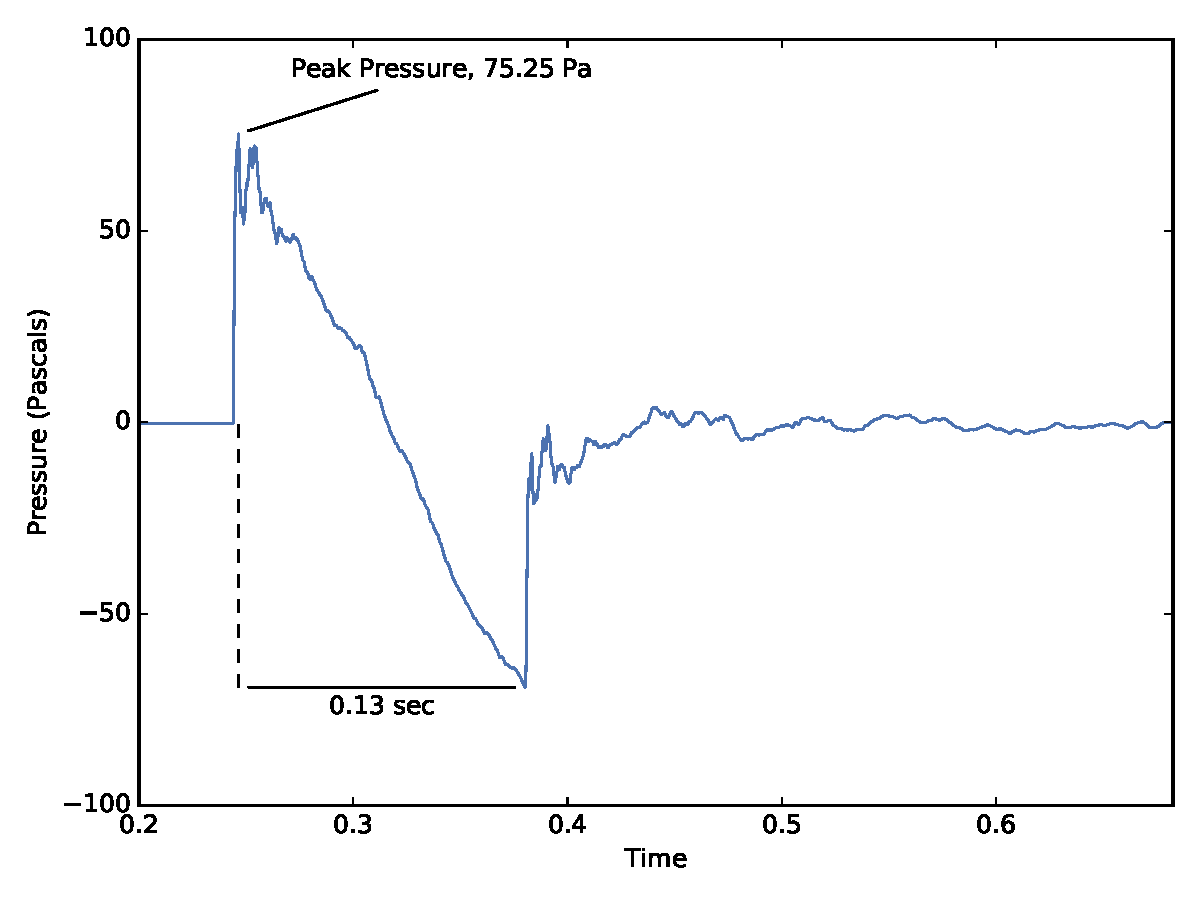
\includegraphics[height=0.5\textheight]{figs/Pascals_vs_Time.pdf}%
  \caption{The waveform in pascals as a function of time. Peak pressure is noted at 75.25 Pa, and the duration in time from the positive-pressure peak to the negative-pressure peak is noted at 0.13 sec.}%
  % \label{fig:fullfig}%
\end{figure*}

\part{[30 pts]} Calculate and plot the single-sided power spectral density function ($G_{xx}$).
\solution

\begin{figure*}[h]
  \centering
  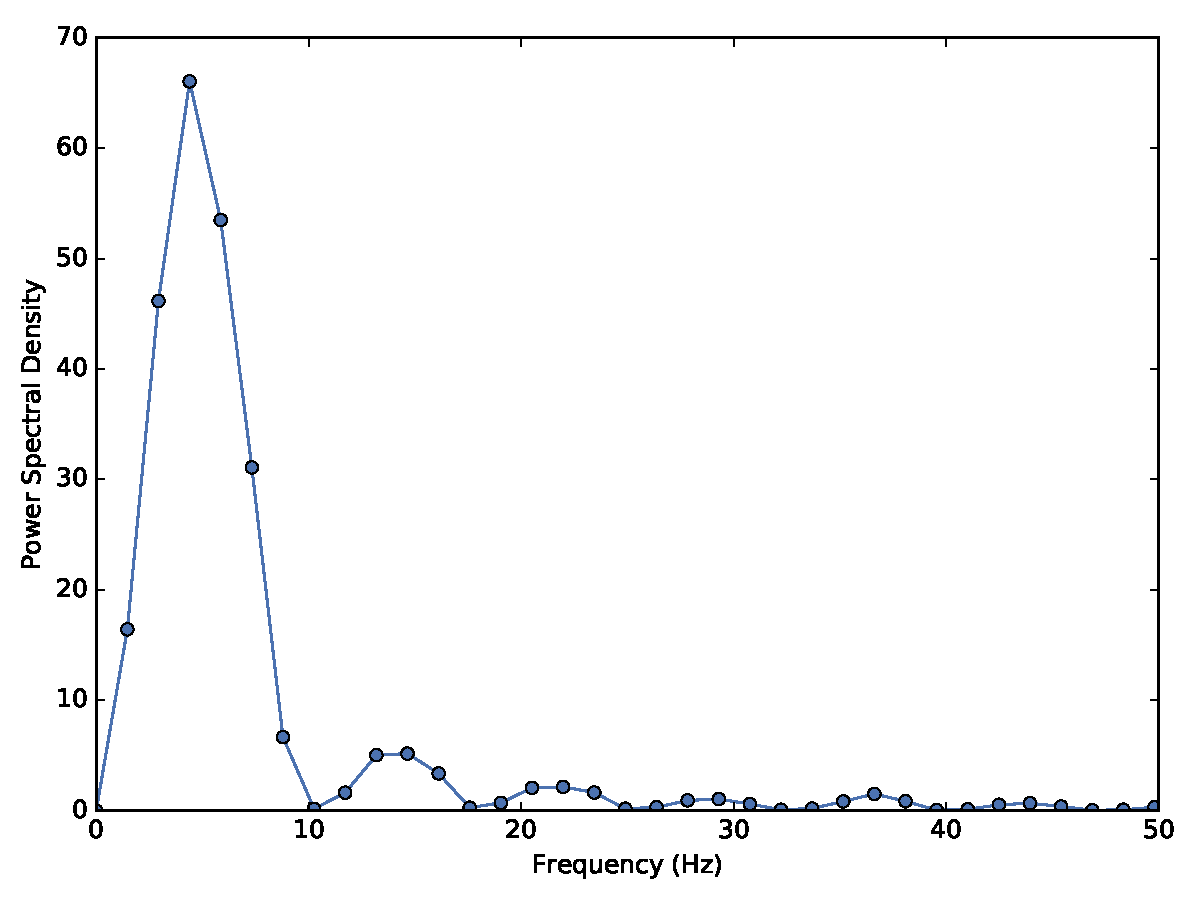
\includegraphics[height=0.3\textheight]{figs/G_xx.pdf}%
  % \caption{The single-sided power spectral density function ($G_{xx}$).}%
  % \label{fig:fullfig}%
\end{figure*}

\part{[10 pts]} Convert and plot the standard narrowband sound pressure level with the reference pressure of 20 micro-Pascal.
\solution

\begin{figure*}[h]
  \centering
  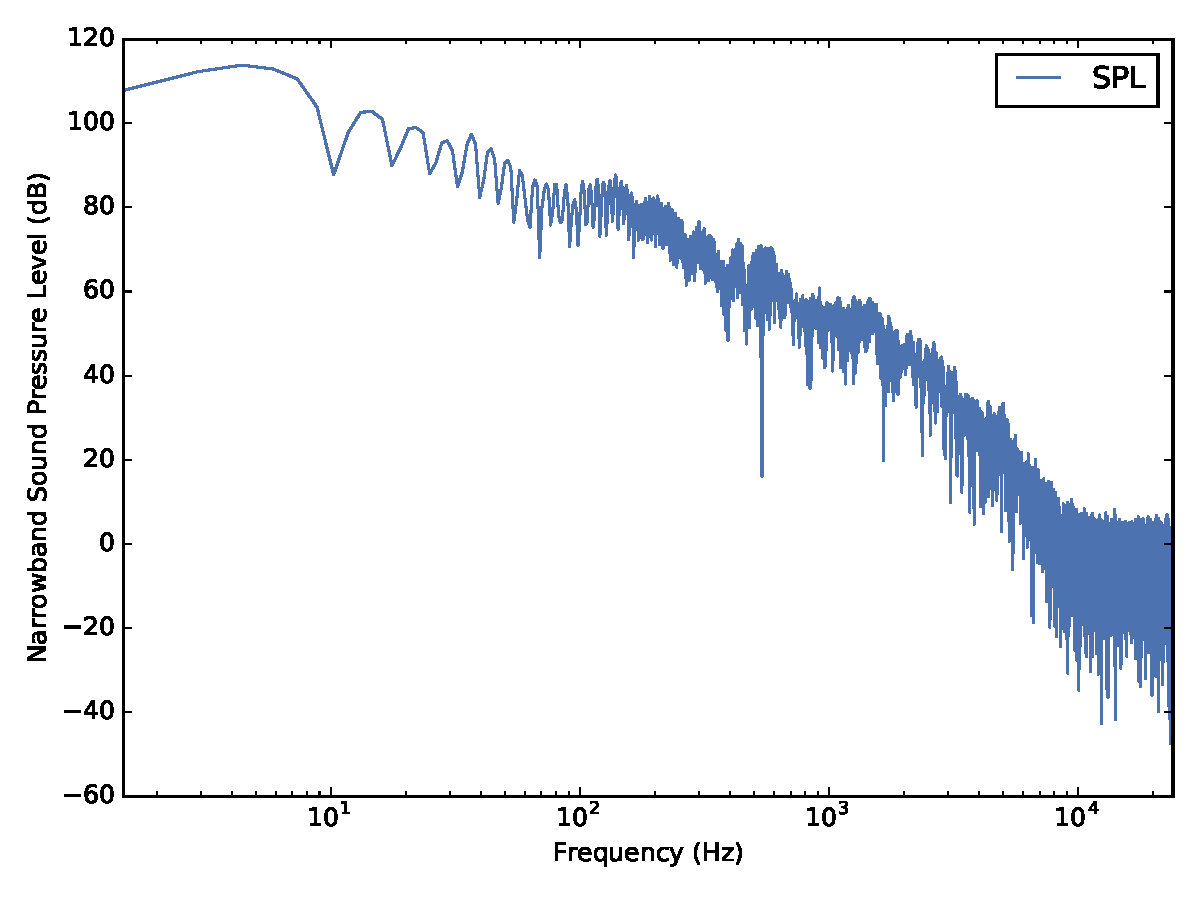
\includegraphics[height=0.3\textheight]{figs/narrowband.pdf}%
  % \caption{The standard narrowband sound pressure level with the reference pressure of 20 micro-Pascal.}%
  % \label{fig:fullfig}%
\end{figure*}

\clearpage
\problem{[50 Pts]} Write a computer program to convert the narrow band spectra to one-third octave and octave band spectra.

[20 pts] Convert the narrowband spectrum to one-third octave band spectrum and make a plot. [20 pts] Convert the one-third octave band spectrum to octave band spectrum and make a plot. [10 pts] Convert the octave band spectrum to the overall sound pressure level.
\solution

\begin{figure*}[h]
  \centering
  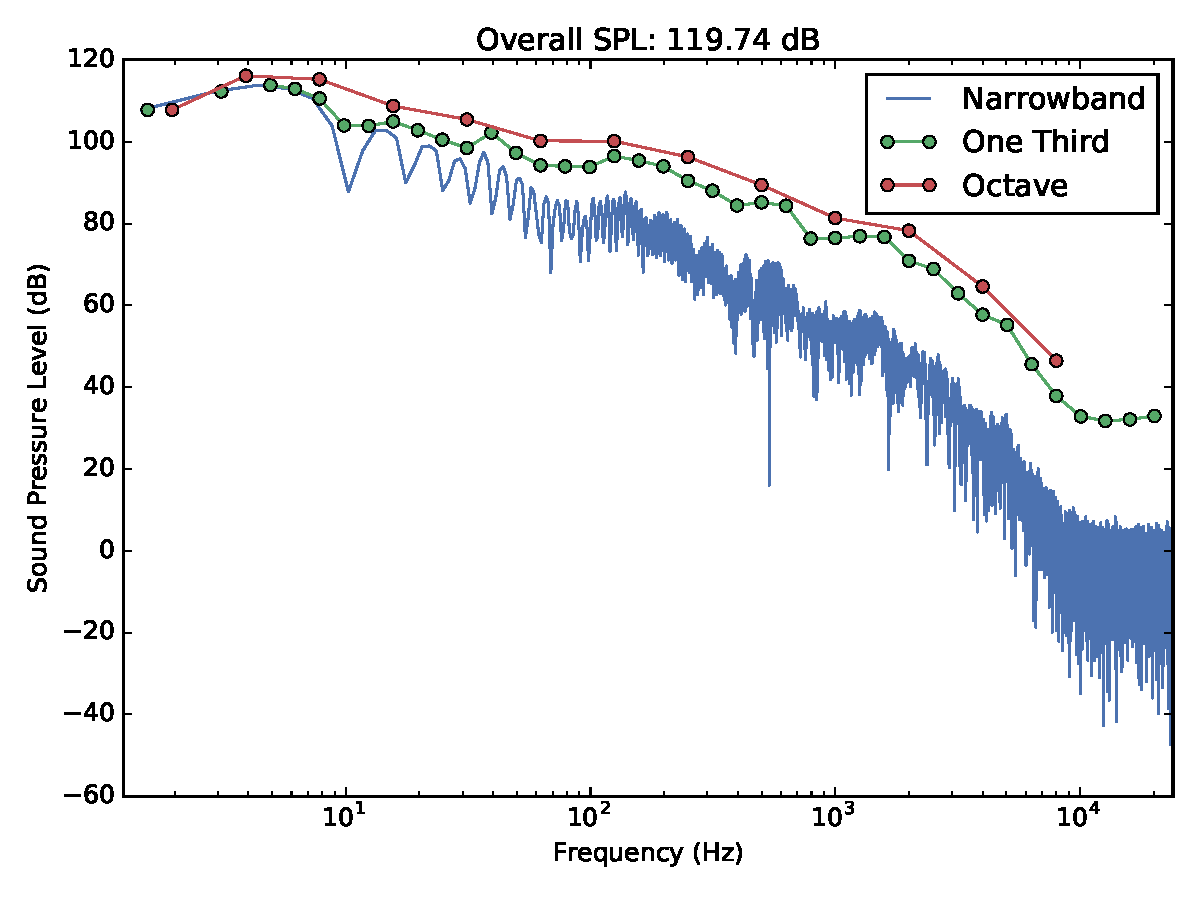
\includegraphics[height=0.5\textheight]{figs/octaves.pdf}%
  \caption{The standard narrowband, 1/3 octave, and octave sound pressure levels with the reference pressure of 20 micro-Pascal. This recording has an overall sound pressure level of 119.74 dB.}%
  % \label{fig:fullfig}%
\end{figure*}

\clearpage
\begin{multicols}{2}
1/3 Octave Results\\

\begin{tabular}{rr}
\toprule
   Frequency (Hz) &         SPL (dB) \\
\midrule
    1.55 &  107.79 \\
    3.10 &  112.28 \\
    4.92 &  113.83 \\
    6.20 &  112.92 \\
    7.81 &  110.56 \\
    9.84 &  103.97 \\
   12.40 &  103.86 \\
   15.62 &  104.95 \\
   19.68 &  102.79 \\
   24.80 &  100.48 \\
   31.25 &   98.47 \\
   39.37 &  102.24 \\
   49.60 &   97.26 \\
   62.50 &   94.23 \\
   78.74 &   93.97 \\
   99.21 &   93.81 \\
  125.00 &   96.48 \\
  157.49 &   95.39 \\
  198.42 &   93.97 \\
  250.00 &   90.44 \\
  314.98 &   88.02 \\
  396.85 &   84.40 \\
  500.00 &   85.15 \\
  629.96 &   84.34 \\
  793.70 &   76.32 \\
 1000.00 &   76.47 \\
 1259.92 &   76.88 \\
 1587.40 &   76.70 \\
 2000.00 &   70.88 \\
 2519.84 &   68.87 \\
 3174.80 &   62.93 \\
 4000.00 &   57.71 \\
 5039.68 &   55.22 \\
 6349.60 &   45.59 \\
 8000.00 &   37.86 \\
10079.36 &   32.84 \\
12699.20 &   31.75 \\
16000.00 &   32.09 \\
20158.73 &   32.95 \\
\bottomrule
\end{tabular}
\\Octave Results\\

\begin{tabular}{rr}
\toprule
Frequency (Hz) &         SPL (dB) \\
\midrule
   1.95 &  107.79 \\
   3.90 &  116.13 \\
   7.81 &  115.24 \\
  15.62 &  108.73 \\
  31.25 &  105.43 \\
  62.50 &  100.20 \\
 125.00 &  100.13 \\
 250.00 &   96.27 \\
 500.00 &   89.42 \\
1000.00 &   81.33 \\
2000.00 &   78.25 \\
4000.00 &   64.60 \\
8000.00 &   46.46 \\
\bottomrule
\end{tabular}
\end{multicols}

\clearpage
\lstinputlisting{../HW1.py}

\end{document}
